% Options for packages loaded elsewhere
\PassOptionsToPackage{unicode,linktoc=all}{hyperref}
\PassOptionsToPackage{hyphens}{url}
\PassOptionsToPackage{dvipsnames,svgnames*,x11names*}{xcolor}
%
\documentclass[
  11pt,
  british,
  a4paper,
]{article}
\usepackage{lmodern}
\usepackage{amsmath}
\usepackage{ifxetex,ifluatex}
\ifnum 0\ifxetex 1\fi\ifluatex 1\fi=0 % if pdftex
  \usepackage[T1]{fontenc}
  \usepackage[utf8]{inputenc}
  \usepackage{textcomp} % provide euro and other symbols
  \usepackage{amssymb}
\else % if luatex or xetex
  \usepackage{unicode-math}
  \defaultfontfeatures{Scale=MatchLowercase}
  \defaultfontfeatures[\rmfamily]{Ligatures=TeX,Scale=1}
\fi
% Use upquote if available, for straight quotes in verbatim environments
\IfFileExists{upquote.sty}{\usepackage{upquote}}{}
\IfFileExists{microtype.sty}{% use microtype if available
  \usepackage[]{microtype}
  \UseMicrotypeSet[protrusion]{basicmath} % disable protrusion for tt fonts
}{}
\makeatletter
\@ifundefined{KOMAClassName}{% if non-KOMA class
  \IfFileExists{parskip.sty}{%
    \usepackage{parskip}
  }{% else
    \setlength{\parindent}{0pt}
    \setlength{\parskip}{6pt plus 2pt minus 1pt}}
}{% if KOMA class
  \KOMAoptions{parskip=half}}
\makeatother
\usepackage{xcolor}
\IfFileExists{xurl.sty}{\usepackage{xurl}}{} % add URL line breaks if available
\IfFileExists{bookmark.sty}{\usepackage{bookmark}}{\usepackage{hyperref}}
\hypersetup{
  pdftitle={Image format conversions},
  pdfauthor={R (Chandra) Chandrasekhar},
  pdflang={en-GB},
  colorlinks=true,
  linkcolor=TealBlue,
  filecolor=Purple,
  citecolor=DarkKhaki,
  urlcolor=Maroon,
  pdfcreator={LaTeX via pandoc}}
\urlstyle{same} % disable monospaced font for URLs
\usepackage[margin=25mm]{geometry}
\usepackage{color}
\usepackage{fancyvrb}
\newcommand{\VerbBar}{|}
\newcommand{\VERB}{\Verb[commandchars=\\\{\}]}
\DefineVerbatimEnvironment{Highlighting}{Verbatim}{commandchars=\\\{\}}
% Add ',fontsize=\small' for more characters per line
\usepackage{framed}
\definecolor{shadecolor}{RGB}{48,48,48}
\newenvironment{Shaded}{\begin{snugshade}}{\end{snugshade}}
\newcommand{\AlertTok}[1]{\textcolor[rgb]{1.00,0.81,0.69}{#1}}
\newcommand{\AnnotationTok}[1]{\textcolor[rgb]{0.50,0.62,0.50}{\textbf{#1}}}
\newcommand{\AttributeTok}[1]{\textcolor[rgb]{0.80,0.80,0.80}{#1}}
\newcommand{\BaseNTok}[1]{\textcolor[rgb]{0.86,0.64,0.64}{#1}}
\newcommand{\BuiltInTok}[1]{\textcolor[rgb]{0.80,0.80,0.80}{#1}}
\newcommand{\CharTok}[1]{\textcolor[rgb]{0.86,0.64,0.64}{#1}}
\newcommand{\CommentTok}[1]{\textcolor[rgb]{0.50,0.62,0.50}{#1}}
\newcommand{\CommentVarTok}[1]{\textcolor[rgb]{0.50,0.62,0.50}{\textbf{#1}}}
\newcommand{\ConstantTok}[1]{\textcolor[rgb]{0.86,0.64,0.64}{\textbf{#1}}}
\newcommand{\ControlFlowTok}[1]{\textcolor[rgb]{0.94,0.87,0.69}{#1}}
\newcommand{\DataTypeTok}[1]{\textcolor[rgb]{0.87,0.87,0.75}{#1}}
\newcommand{\DecValTok}[1]{\textcolor[rgb]{0.86,0.86,0.80}{#1}}
\newcommand{\DocumentationTok}[1]{\textcolor[rgb]{0.50,0.62,0.50}{#1}}
\newcommand{\ErrorTok}[1]{\textcolor[rgb]{0.76,0.75,0.62}{#1}}
\newcommand{\ExtensionTok}[1]{\textcolor[rgb]{0.80,0.80,0.80}{#1}}
\newcommand{\FloatTok}[1]{\textcolor[rgb]{0.75,0.75,0.82}{#1}}
\newcommand{\FunctionTok}[1]{\textcolor[rgb]{0.94,0.94,0.56}{#1}}
\newcommand{\ImportTok}[1]{\textcolor[rgb]{0.80,0.80,0.80}{#1}}
\newcommand{\InformationTok}[1]{\textcolor[rgb]{0.50,0.62,0.50}{\textbf{#1}}}
\newcommand{\KeywordTok}[1]{\textcolor[rgb]{0.94,0.87,0.69}{#1}}
\newcommand{\NormalTok}[1]{\textcolor[rgb]{0.80,0.80,0.80}{#1}}
\newcommand{\OperatorTok}[1]{\textcolor[rgb]{0.94,0.94,0.82}{#1}}
\newcommand{\OtherTok}[1]{\textcolor[rgb]{0.94,0.94,0.56}{#1}}
\newcommand{\PreprocessorTok}[1]{\textcolor[rgb]{1.00,0.81,0.69}{\textbf{#1}}}
\newcommand{\RegionMarkerTok}[1]{\textcolor[rgb]{0.80,0.80,0.80}{#1}}
\newcommand{\SpecialCharTok}[1]{\textcolor[rgb]{0.86,0.64,0.64}{#1}}
\newcommand{\SpecialStringTok}[1]{\textcolor[rgb]{0.80,0.58,0.58}{#1}}
\newcommand{\StringTok}[1]{\textcolor[rgb]{0.80,0.58,0.58}{#1}}
\newcommand{\VariableTok}[1]{\textcolor[rgb]{0.80,0.80,0.80}{#1}}
\newcommand{\VerbatimStringTok}[1]{\textcolor[rgb]{0.80,0.58,0.58}{#1}}
\newcommand{\WarningTok}[1]{\textcolor[rgb]{0.50,0.62,0.50}{\textbf{#1}}}
\usepackage{graphicx}
\makeatletter
\def\maxwidth{\ifdim\Gin@nat@width>\linewidth\linewidth\else\Gin@nat@width\fi}
\def\maxheight{\ifdim\Gin@nat@height>\textheight\textheight\else\Gin@nat@height\fi}
\makeatother
% Scale images if necessary, so that they will not overflow the page
% margins by default, and it is still possible to overwrite the defaults
% using explicit options in \includegraphics[width, height, ...]{}
\setkeys{Gin}{width=\maxwidth,height=\maxheight,keepaspectratio}
% Set default figure placement to htbp
\makeatletter
\def\fps@figure{htbp}
\makeatother
\setlength{\emergencystretch}{3em} % prevent overfull lines
\providecommand{\tightlist}{%
  \setlength{\itemsep}{0pt}\setlength{\parskip}{0pt}}
\setcounter{secnumdepth}{-\maxdimen} % remove section numbering
\AtBeginEnvironment{quote}{\small}
\setlength{\parindent}{0pt} % block paragraphs
\usepackage{etoolbox}
\usepackage{graphicx}
\usepackage{subcaption}
\usepackage{svg}
\usepackage[Latin,Tamil,Devanagari]{ucharclasses}
  \setmainfont[SmallCapsFont={Charis SIL Small Caps}]{Charis SIL}
  \setsansfont[Numbers=OldStyle,BoldFont={* Semibold}]{Source Sans Pro}
  \setmonofont[Scale=0.90]{Fira Mono}
  \defaultfontfeatures{Ligatures=TeX,Scale=MatchLowercase}
  \setmathfont[bold-style=ISO]{STIX Two Math}
  \newfontfamily\tamilfont[Script=Tamil]{Noto Sans Tamil}
  \setTransitionsFor{Tamil}{\tamilfont}{\normalfont}
  \setTransitionTo{Tamil}{\tamilfont}{}
  \setTransitionFrom{Tamil}{\normalfont}
  \newfontfamily\devfont[Script=Devanagari]{Noto Sans Devanagari}
  \setTransitionsFor{Devanagari}{\devfont}{\normalfont}
  \setTransitionTo{Devanagari}{\devfont}{}
  \setTransitionFrom{Devanagari}{\normalfont}
  \newfontfamily{\emojifont}{Symbola}
\usepackage[all]{nowidow}
\usepackage[margins=raggedright]{floatrow}
%
% Tables without rules
%
\let\addlinespace\relax
\let\toprule\relax
\let\bottomrule\relax
\let\midrule\relax
\let\addlinespace\relax
%
% Adjust punctuation for footnotes
%
\usepackage{fnpct} % footnote _before_ punctuation reversed and adjusted.
  \setfnpct{after-dot-space=-0.15em,after-comma-space=-0.150em,add-punct-marks=;[0.06em]![0.06em]?[0.06em]:[0.06em]}
%
% Flexible fontsizes
%
\usepackage{fontsize}
%
\usepackage{titling}
\usepackage{fancyhdr}
    \pagestyle{fancy}
    \fancyhead{}
    \fancyfoot{}
    \renewcommand{\headrulewidth}{0.2pt}
    \renewcommand{\footrulewidth}{0.2pt}
    \fancyhead[LO,RE]{\scshape\thetitle}
    \fancyfoot[CO,CE]{\small Copyright © 2006--\the\year, R (Chandra) Chandrasekhar}
    \fancyfoot[RE,RO]{\thepage}
%% pandoc-eqnos
\usepackage[capitalise]{cleveref}
  \crefname{equation}{Equation}{Equations}
  \crefname{figure}{Figure}{Figures}
%% pandoc-fignos
\usepackage{caption}
%% pandoc-fignos: environment to disable figure caption prefixes
    \makeatletter
    \newcounter{figno}
    \newenvironment{fignos:no-prefix-figure-caption}{
      \caption@ifcompatibility{}{
        \let\oldthefigure\thefigure
        \let\oldtheHfigure\theHfigure
        \renewcommand{\thefigure}{figno:\thefigno}
        \renewcommand{\theHfigure}{figno:\thefigno}
        \stepcounter{figno}
        \captionsetup{labelformat=empty}
      }
    }{
      \caption@ifcompatibility{}{
        \captionsetup{labelformat=default}
        \let\thefigure\oldthefigure
        \let\theHfigure\oldtheHfigure
        \addtocounter{figure}{-1}
      }
    }
    \makeatother
%%

\ifxetex
  % Load polyglossia as late as possible: uses bidi with RTL langages (e.g. Hebrew, Arabic)
  \usepackage{polyglossia}
  \setmainlanguage[variant=british]{english}
\else
  \usepackage[shorthands=off,main=british]{babel}
\fi
\ifluatex
  \usepackage{selnolig}  % disable illegal ligatures
\fi
\newlength{\cslhangindent}
\setlength{\cslhangindent}{1.5em}
\newlength{\csllabelwidth}
\setlength{\csllabelwidth}{3em}
\newenvironment{CSLReferences}[2] % #1 hanging-ident, #2 entry spacing
 {% don't indent paragraphs
  \setlength{\parindent}{0pt}
  % turn on hanging indent if param 1 is 1
  \ifodd #1 \everypar{\setlength{\hangindent}{\cslhangindent}}\ignorespaces\fi
  % set entry spacing
  \ifnum #2 > 0
  \setlength{\parskip}{#2\baselineskip}
  \fi
 }%
 {}
\usepackage{calc}
\newcommand{\CSLBlock}[1]{#1\hfill\break}
\newcommand{\CSLLeftMargin}[1]{\parbox[t]{\csllabelwidth}{#1}}
\newcommand{\CSLRightInline}[1]{\parbox[t]{\linewidth - \csllabelwidth}{#1}\break}
\newcommand{\CSLIndent}[1]{\hspace{\cslhangindent}#1}

\title{Image format conversions}
\author{R (Chandra) Chandrasekhar}
\date{2021-03-07 | 2021-03-07}

\begin{document}
\maketitle

\thispagestyle{empty}


\hypertarget{two-varieties-of-digital-images}{%
\subsection{Two varieties of digital
images}\label{two-varieties-of-digital-images}}

Digital images come in two broad flavours:

\begin{itemize}
\tightlist
\item
  \href{https://en.wikipedia.org/wiki/Raster_graphics}{raster} or
  \href{https://en.wikipedia.org/wiki/Bitmap}{bitmap} graphics, and
\item
  \href{https://en.wikipedia.org/wiki/Vector_graphics}{vector graphics}.
\end{itemize}

The former leads to image blockiness or
\href{https://en.wikipedia.org/wiki/Pixelation}{pixellation} at high
magnifications, as shown in \cref{fig:raster}, while the latter scales
without degradation when magnified, as illustrated in \cref{fig:vector}.

\begin{figure}
\hypertarget{fig:raster}{%
\centering
\includegraphics[width=0.5\textwidth,height=\textheight]{images/raster.png}
\caption{Raster graphics image of the letter O (PNG
format)}\label{fig:raster}
}
\end{figure}

\begin{figure}
\hypertarget{fig:vector}{%
\centering
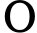
\includegraphics[width=0.5\textwidth,height=\textheight]{images/vector.svg}
\caption{Vector graphics image of the letter O (SVG
format)}\label{fig:vector}
}
\end{figure}

\hypertarget{raster-graphics}{%
\subsubsection{Raster Graphics}\label{raster-graphics}}

There are dozens of image formats, including these three:

\begin{enumerate}
\tightlist
\item
  \href{https://en.wikipedia.org/wiki/TIFF}{Tag(ged) Image File Format
  (TIFF)}

  \begin{itemize}
  \tightlist
  \item
    lossless compression
  \item
    large file sizes
  \item
    used in printing and professional graphics
  \item
    preferred for archival of scanned photographs
  \end{itemize}
\item
  \href{https://jpeg.org/about.html}{Joint Photographic Experts Group
  (JPEG)} format

  \begin{itemize}
  \tightlist
  \item
    small file sizes
  \item
    lossy compression
  \item
    good quality with fast downloads
  \item
    supported by web browsers
  \item
    preferred for scenes and portraits
  \item
    no transparency
  \end{itemize}
\item
  \href{http://www.libpng.org/pub/png/}{Portable Network Graphics (PNG)}
  format

  \begin{itemize}
  \tightlist
  \item
    lossless compression
  \item
    preferred for text and high definition images
  \item
    supported by most web browsers
  \item
    transparency
  \end{itemize}
\end{enumerate}

All three formats employ raster graphics in which image elements are
represented as rectangular arrays of
\href{https://en.wikipedia.org/wiki/Pixels}{pixels}.

\hypertarget{vector-graphics}{%
\subsubsection{Vector Graphics}\label{vector-graphics}}

The two principal vector graphics formats are:

\begin{enumerate}
\tightlist
\item
  \href{https://en.wikipedia.org/wiki/PDF}{Portable Document Format
  (PDF)}

  \begin{itemize}
  \tightlist
  \item
    preferred for archival quality electronic and printed documents
  \item
    supported by browsers with integrated PDF readers
  \item
    file sizes comparable to raster images
  \item
    machine-readable files
  \end{itemize}
\item
  \href{https://en.wikipedia.org/wiki/Scalable_Vector_Graphics}{Scalable
  Vector Graphics (SVG)} format

  \begin{itemize}
  \tightlist
  \item
    preferred for scalable graphics on web browsers
  \item
    used in digital image animations and digital art
  \item
    small file sizes
  \item
    human- and machine-readable files
  \end{itemize}
\end{enumerate}

Both these formats yield images which consist of mathematically defined
points, lines, curves, and shapes.

\hypertarget{format-conversions}{%
\subsection{Format conversions}\label{format-conversions}}

For a variety of reasons, it is often necessary to convert from one
image format to another. There are four broad possibilities for this:

\begin{enumerate}
\def\labelenumi{\alph{enumi}.}
\tightlist
\item
  raster to raster;
\item
  raster to vector;
\item
  vector to raster; and
\item
  vector to vector
\end{enumerate}

We consider each of these in turn using
\href{https://itlaw.wikia.org/wiki/Platform_neutral}{platform-neutral}
\href{https://opensource.com/resources/what-open-source}{open source}
tools. Since I run
\href{https://en.wikipedia.org/wiki/GNU/Linux_naming_controversy}{GNU/Linux}
on my desktop, my examples will feature commands from that
setup.\footnote{There are many websites that promise conversion online,
  requiring you to upload the input file and download the output file.
  These \emph{might be} fraught with security risks. Use them with
  caution.}

\hypertarget{tools-for-image-format-conversion}{%
\subsection{Tools for image format
conversion}\label{tools-for-image-format-conversion}}

Among the very many tools available, we examine below four that support
image format conversion:

\begin{enumerate}
\tightlist
\item
  \href{https://imagemagick.org/index.php}{ImageMagick}

  \begin{itemize}
  \tightlist
  \item
    graphics library for image manipulation and display
  \item
    standalone utilities like \texttt{convert}, \texttt{display},
    \texttt{identify}, \texttt{mogrify}, etc.
  \item
    scripting language
  \item
    pixel-based
  \item
    raster to raster conversions
  \item
    raster to vector conversions
  \end{itemize}
\item
  \href{https://www.cairographics.org/}{cairo}

  \begin{itemize}
  \tightlist
  \item
    vector-based 2D drawing and rendering library
  \item
    multiple output devices/formats
  \item
    used by other programs rather than in standalone mode
  \end{itemize}
\item
  \href{https://poppler.freedesktop.org/}{poppler}

  \begin{itemize}
  \tightlist
  \item
    vector-based PDF rendering library
  \item
    used by several PDF viewers
  \item
    uses cairo as backend
  \item
    standalone utilities like \texttt{pdftotext}, \texttt{pdftocairo},
    and \texttt{pdftoppm}
  \end{itemize}
\item
  \href{https://inkscape.org/}{Inkscape}

  \begin{itemize}
  \tightlist
  \item
    GUI-based vector graphics editor
  \item
    suitable both for technical illustration and digital art
  \item
    uses SVG as the main format
  \item
    can export to a wide variety of output formats
  \item
    option to use cairo for PDF export
  \end{itemize}
\end{enumerate}

\hypertarget{imagemagick-the-swiss-army-knife}{%
\subsection{ImageMagick: the Swiss Army
knife}\label{imagemagick-the-swiss-army-knife}}

ImageMagick is the name given to a suite of image processing tools
originally created in 1987 by John Cristy, then working for
\href{https://www.dupont.com/}{Du Pont}. In 1990, it was freely released
by Du Pont, who transferred copyright to
\href{https://imagemagick.org/script/contact.php}{ImageMagick Studio
LLC} who now maintain the project. It is distributed under a derived
Apache 2.0 \href{https://imagemagick.org/script/license.php}{license}.
The \href{https://github.com/ImageMagick/ImageMagick}{authoritative
source code repository} shows active development even today, 34 years
after the suite was first released {[}1{]}.

ImageMagick is so versatile and useful that it may rightfully be called
the \href{https://www.thefreedictionary.com/Swiss-army+knife}{Swiss Army
knife} of the image processing world. It comes with several command line
utilities, each replete with options. Among these are:

\begin{itemize}
\tightlist
\item
  \href{https://imagemagick.org/script/convert.php}{\texttt{convert}}
  which converts from one format to another;
\item
  \href{https://imagemagick.org/script/display.php}{\texttt{display}}
  which displays one or more images;
\item
  \href{https://imagemagick.org/script/identify.php}{\texttt{identify}}
  which identifies the type of image and displays its characteristics;
\item
  \href{https://imagemagick.org/script/mogrify.php}{\texttt{mogrify}}
  which transforms an image, modifying its appearance; and
\item
  \href{https://imagemagick.org/script/montage.php}{\texttt{montage}}
  which generates an image montage from several images.
\end{itemize}

The above list is far from exhaustive. The interested reader is referred
to the
\href{https://imagemagick.org/script/command-line-tools.php}{excellent
online documentation} for further details. The power of ImageMagick is
enhanced with the
\href{https://imagemagick.org/script/magick-script.php}{magick-script}
Image Scripting Language. The examples in this blog use the command line
versions of invoking ImageMagick. If they seem daunting,
\href{https://imagemagick.org/script/command-line-processing.php}{refer
to this explanation} {[}2{]}.

\hypertarget{test-images}{%
\subsection{Test images}\label{test-images}}

Two quite different images are used to illustrate the format conversions
we perform here. The two test images are:

\begin{enumerate}
\tightlist
\item
  a coloured, text-only test image called \texttt{text-only.png}; and
\item
  a non-text, coloured, graphically rich image called
  \texttt{animals.jpg}.
\end{enumerate}

We will refer to these two images as \texttt{text-only} and
\texttt{animals}, respectively hereafter.

\hypertarget{text-only-image}{%
\subsubsection{Text-only image}\label{text-only-image}}

The \texttt{text-only} image was first generated as a PDF file,
\texttt{text-only.pdf}, by compiling a
\href{https://www.latex-project.org/}{LaTeX} source file. That file was
then converted to various raster formats using the methods
\protect\hyperlink{vector-to-raster}{discussed later} to yield the
images \texttt{text-only-600-dpi.png} and
\texttt{text-only-600-dpi.jpg}.

\begin{figure}
\hypertarget{fig:text-only}{%
\centering
\includegraphics[width=0.8\textwidth,height=\textheight]{images/text-only-600-dpi-cairo.png}
\caption{Text-only image in PNG format.}\label{fig:text-only}
}
\end{figure}

\hypertarget{non-text-test-image}{%
\subsubsection{Non-text test image}\label{non-text-test-image}}

The non-text \texttt{animals} image is a colourful, graphically rich
image with much detail. It is from a hand-drawn illustration of
microscopic marine animals by the German naturalist
\href{https://en.wikipedia.org/wiki/Ernst_Haeckel}{Ernst Haeckel},
scanned as a JPEG, and made available in the public domain.

\begin{figure}
\hypertarget{fig:animals}{%
\centering
\includegraphics[width=0.8\textwidth,height=\textheight]{images/animals.jpg}
\caption[Non-text, graphically rich \texttt{animals} image in JPEG
format.]{Non-text, graphically rich \texttt{animals} image in JPEG
format.\footnotemark{}}\label{fig:animals}
}
\end{figure}
\footnotetext{These images are in the public domain and covered by the
  \href{https://creativecommons.org/publicdomain/zero/1.0/}{CC0
  licence}. They are available for download
  \href{https://www.rawpixel.com/image/2266608/free-illustration-image-ernst-haeckel-vintage-animals}{here}.}

\hypertarget{pre-processing-cropping}{%
\subsection{Pre-processing: Cropping}\label{pre-processing-cropping}}

Cropping is strictly not image format conversion, but is often a
necessary pre-processing step in image manipulations. For example,
\cref{fig:animals} has a whitish, non-monochromatic border around the
block print, containing annotations. For our purposes, this border is
more of a distraction that is best removed altogether by
\emph{cropping}, leaving us with only the illustration. We will refer to
the cropped image as \texttt{animals-cropped} and use it as the source
image in our examples below.

Cropping is usually better done interactively using a
\href{https://en.wikipedia.org/wiki/Graphical_user_interface}{GUI
(Graphical User Interface)}, than on the command line. The latter, even
if a bit tedious, is precisely repeatable.

ImageMagick's \texttt{display} utility pops up a GUI with a left click
when the mouse is over the image. We can then drag and fit a window to
the \emph{region we wish to keep}, clicking the crop function, and
saving the cropped image. The steps are these:

\begin{enumerate}
\def\labelenumi{\alph{enumi}.}
\tightlist
\item
  left mouse click on the image to reveal the GUI (see \cref{fig:gui});
\item
  \texttt{Transform\ -\textgreater{}\ Crop};
\item
  put the mouse over the top left corner and drag until the bottom right
  corner to enclose the region of interest;
\item
  Click again on \texttt{Crop}; and
\item
  \texttt{File\ -\textgreater{}\ Save} with a different name.
\end{enumerate}

\begin{figure}
\hypertarget{fig:gui}{%
\centering
\includegraphics[width=0.2\textwidth,height=\textheight]{images/ImageMagick-display-gui.png}
\caption{ImageMagick interactive GUI.}\label{fig:gui}
}
\end{figure}

Alternatively, we may just position the cursor on the top left and
bottom right corners of the region we wish to \emph{retain}, noting the
co-ordinates in each case. If these coordinates are \((x_t, y_t)\) and
\((x_b, y_b)\), respectively, we have \(w = x_b - x_t\) and
\(h = y_b -y_t\). We may then invoke the convert command with crop as
the option so:

\begin{Shaded}
\begin{Highlighting}[]
\ExtensionTok{convert} \AttributeTok{{-}crop} \StringTok{\textquotesingle{}wxh+x\_t+y\_t\textquotesingle{}}\NormalTok{ animals.jpg animals{-}cropped.jpg}
\end{Highlighting}
\end{Shaded}

In our case, \((x_t, y_t) = (60, 84)\) and \((x_b, y_b) = (795, 1119)\)
giving \(w = 735\) and \(h = 1035\), leading to

\begin{Shaded}
\begin{Highlighting}[]
\ExtensionTok{convert} \AttributeTok{{-}crop} \StringTok{\textquotesingle{}735x1035+60+84\textquotesingle{}}\NormalTok{ animals.jpg animals{-}cropped.jpg}
\end{Highlighting}
\end{Shaded}

The resulting cropped image is shown in \cref{fig:cropped} below.

\begin{figure}
\hypertarget{fig:cropped}{%
\centering
\includegraphics[width=0.5\textwidth,height=\textheight]{images/test-cropped.jpg}
\caption{Cropped version of the image in
\cref{fig:test}.}\label{fig:cropped}
}
\end{figure}

\hypertarget{file-sizes}{%
\subsubsection{File sizes}\label{file-sizes}}

The sizes of the original and cropped files are shown below in human
friendly numbers:

\begin{Shaded}
\begin{Highlighting}[]
\FunctionTok{ls} \AttributeTok{{-}sh}\NormalTok{ animals}\PreprocessorTok{*}\NormalTok{.jpg }\KeywordTok{|} \FunctionTok{awk} \StringTok{\textquotesingle{}\{print $1 "\textbackslash{}t" $2\}\textquotesingle{}}
\ExtensionTok{{-}{-}{-}}
\ExtensionTok{200K}\NormalTok{    animals{-}cropped.jpg}
\ExtensionTok{312K}\NormalTok{    animals.jpg}
\end{Highlighting}
\end{Shaded}

As expected, the original file \texttt{animals.jpg} is larger than the
cropped full-size version, \texttt{animals-cropped.jpg} and all is well.

\hypertarget{raster-to-raster-conversion}{%
\subsection{Raster to raster
conversion}\label{raster-to-raster-conversion}}

We now perform a sequence of image manipulations, including raster to
raster format conversions.

\hypertarget{resizing-format-conversion-and-montaging}{%
\subsubsection{Resizing, format-conversion, and
montaging}\label{resizing-format-conversion-and-montaging}}

We may invoke ImageMagick's \texttt{convert} function not only to
convert from one format to another but also to accomplish cropping (as
we have already seen), image-resizing, making the background
transparent, and
\href{https://www.thefreedictionary.com/montage}{montaging}, etc.

Suppose we want to reduce the dimensions of the cropped image to half
their original values, and display the full-size and half-size images
side by side, we could run the following command:

\begin{Shaded}
\begin{Highlighting}[]
\ExtensionTok{convert}\NormalTok{ animals{-}cropped.jpg }\AttributeTok{{-}resize}\NormalTok{ 50\% animals{-}cropped{-}halfsize.jpg}

\ExtensionTok{convert}\NormalTok{ animals{-}cropped.jpg +append }\AttributeTok{{-}gravity}\NormalTok{ south }\DataTypeTok{\textbackslash{}}
\NormalTok{animals{-}cropped{-}halfsize.jpg both.jpg}
\end{Highlighting}
\end{Shaded}

\begin{figure}
\hypertarget{fig:both-jpg}{%
\centering
\includegraphics[width=0.8\textwidth,height=\textheight]{images/both.jpg}
\caption{Full-size cropped image on the left and half-sized image on the
right.}\label{fig:both-jpg}
}
\end{figure}

\hypertarget{background-transparency}{%
\subsubsection{Background transparency}\label{background-transparency}}

Notice that there is a coloured white rectangle atop the half-size image
on the right in \cref{fig:both-jpg}. We could remove it by rendering the
background transparent, but because JPEG does not support transparency,
through an
\href{https://www.techopedia.com/definition/1945/alpha-channel}{alpha
channel}, we have to convert the composite image to the PNG format,
which does. This is one real-life circumstance necessitating raster to
raster format conversion.

\begin{Shaded}
\begin{Highlighting}[]
\ExtensionTok{convert}\NormalTok{ +append }\AttributeTok{{-}gravity}\NormalTok{ south }\AttributeTok{{-}background}\NormalTok{ transparent }\DataTypeTok{\textbackslash{}}
\NormalTok{animals{-}cropped.jpg animals{-}cropped{-}halfsize.jpg both.png}
\end{Highlighting}
\end{Shaded}

\begin{figure}
\hypertarget{fig:both-png}{%
\centering
\includegraphics[width=0.8\textwidth,height=\textheight]{images/both.png}
\caption{Composite image converted to PNG format with transparent
background.}\label{fig:both-png}
}
\end{figure}

\hypertarget{file-sizes-again}{%
\paragraph{File sizes again}\label{file-sizes-again}}

How do the file sizes of the two composite images compare? How high a
price have we paid for the transparent background?

\begin{Shaded}
\begin{Highlighting}[]
\FunctionTok{ls} \AttributeTok{{-}sh}\NormalTok{ both.}\PreprocessorTok{*} \KeywordTok{|} \FunctionTok{awk} \StringTok{\textquotesingle{}\{print $1 "\textbackslash{}t" $2\}\textquotesingle{}}

\ExtensionTok{264K}\NormalTok{    both.jpg}
\ExtensionTok{2.2M}\NormalTok{    both.png}
\end{Highlighting}
\end{Shaded}

And the shocker is clearly shown above. The PNG composite image is
\emph{almost eight times larger} than its JPEG counterpart.

\hypertarget{compression-levels-and-file-sizes}{%
\paragraph{Compression levels and file
sizes}\label{compression-levels-and-file-sizes}}

The \href{https://en.wikipedia.org/wiki/Image_compression}{image
compression level} used above is the default compression level in
ImageMagick. Getting the right combination of image dimensions, image
compression, and image quality so that the image loads fast and looks
good is
\href{https://www.smashingmagazine.com/2015/06/efficient-image-resizing-with-imagemagick/}{quite
an art}. {[}3{]}

To get an idea of the range of file sizes involved, let us try
generating a composite image with extremes of the compression level,
which can range from 0 to 9.

\begin{Shaded}
\begin{Highlighting}[]
\ExtensionTok{convert} \AttributeTok{{-}define}\NormalTok{ PNG:compression{-}level=0 +append }\AttributeTok{{-}gravity}\NormalTok{ south }\DataTypeTok{\textbackslash{}}
\NormalTok{{-}background transparent }\DataTypeTok{\textbackslash{}}
\NormalTok{animals{-}cropped.jpg animals{-}cropped{-}halfsize.jpg }\DataTypeTok{\textbackslash{}}
\NormalTok{both{-}compressed{-}0.png}

\ExtensionTok{convert} \AttributeTok{{-}define}\NormalTok{ PNG:compression{-}level=9 +append }\AttributeTok{{-}gravity}\NormalTok{ south }\DataTypeTok{\textbackslash{}}
\NormalTok{{-}background transparent }\DataTypeTok{\textbackslash{}}
\NormalTok{animals{-}cropped.jpg animals{-}cropped{-}halfsize.jpg }\DataTypeTok{\textbackslash{}}
\NormalTok{both{-}compressed{-}9.png}
\end{Highlighting}
\end{Shaded}

The file sizes are:

\begin{Shaded}
\begin{Highlighting}[]
\FunctionTok{ls} \AttributeTok{{-}sh}\NormalTok{ both}\PreprocessorTok{*} \KeywordTok{|} \FunctionTok{awk} \StringTok{\textquotesingle{}\{print $1 "\textbackslash{}t" $2\}\textquotesingle{}}
\ExtensionTok{{-}{-}{-}}
\ExtensionTok{4.4M}\NormalTok{    both{-}compressed{-}0.png}
\ExtensionTok{2.2M}\NormalTok{    both{-}compressed{-}9.png}
\ExtensionTok{4.4M}\NormalTok{    both{-}compressed.png}
\ExtensionTok{264K}\NormalTok{    both.jpg}
\ExtensionTok{2.2M}\NormalTok{    both.png}
\end{Highlighting}
\end{Shaded}

It appears that the default compression used by ImageMagick gives a file
size that is the same as the highest compression level. Indeed, the
uncompressed version---with a compression level of zero---gives a file
\emph{twice} the size of the uncompressed version and \emph{sixteen
times} the size of the JPEG. And we have not even used two other related
attributes:
\href{https://stackoverflow.com/questions/27267073/imagemagick-lossless-max-compression-for-png}{filter
and strategy} {[}4{]}. Getting the best tradeoff of image size, file
size, loading time, and image quality is still more an art to be
mastered than an algorithm to be applied.

\hypertarget{results-with-the-text-only-image}{%
\subsubsection{Results with the text-only
image}\label{results-with-the-text-only-image}}

For completeness, let us do a simple \emph{no quality loss} conversion
from PNG to JPEG for the text-only test image, and compare image
appearances and file sizes.

\begin{Shaded}
\begin{Highlighting}[]
\ExtensionTok{convert} \AttributeTok{{-}quality}\NormalTok{ 100 text{-}only{-}600{-}dpi{-}cairo.png text{-}only{-}600{-}dpi{-}cairo.jpg}

\ExtensionTok{convert}\NormalTok{ text{-}only{-}600{-}dpi{-}cairo.png text{-}only{-}600{-}dpi{-}cairo.jpg }\DataTypeTok{\textbackslash{}}
\NormalTok{{-}background transparent }\AttributeTok{{-}splice}\NormalTok{ 20x0+0+0 +append }\AttributeTok{{-}chop}\NormalTok{ 20x0+0+0 }\DataTypeTok{\textbackslash{}}
\NormalTok{text{-}only{-}both{-}600{-}dpi{-}cairo.png}

\FunctionTok{ls} \AttributeTok{{-}Xsh}\NormalTok{ text}\PreprocessorTok{*}\NormalTok{cairo}\PreprocessorTok{*} \KeywordTok{|} \FunctionTok{awk} \StringTok{\textquotesingle{}\{print $1 "\textbackslash{}t" $2\}\textquotesingle{}}
\ExtensionTok{{-}{-}{-}}
\ExtensionTok{148K}\NormalTok{    text{-}only{-}600{-}dpi{-}cairo.jpg}
\ExtensionTok{40K}\NormalTok{     text{-}only{-}600{-}dpi{-}cairo.png}
\ExtensionTok{120K}\NormalTok{    text{-}only{-}both{-}600{-}dpi{-}cairo.png}
\end{Highlighting}
\end{Shaded}

\begin{figure}
\hypertarget{fig:text-only-both}{%
\centering
\includegraphics[width=0.8\textwidth,height=\textheight]{images/text-only-both-600-dpi-cairo.png}
\caption{Composite of the PNG on the left, and JPEG on the right, with a
small separator.}\label{fig:text-only-both}
}
\end{figure}

\Cref{fig:text-only-both} does not reveal any degradation in quality
after conversion from PNG to JPEG. Note also that the \emph{composite}
PNG image is smaller than the \emph{single} JPEG image. We
conclude---rather shakily on the basis of one instance---that PNG is
better suited for textual images and provides a smaller file size for
the same quality.

XXXXX Need to compare with original pdfto jpeg and using convert to get
jpeg

\hypertarget{can-cairo-and-poppler-do-all-this}{%
\subsubsection{Can cairo and poppler do all
this?}\label{can-cairo-and-poppler-do-all-this}}

Can such processing be done using cairo or poppler? Not really. The
\emph{starting point} or \emph{input format} for cairo and poppler is
the PDF format. Our test image is scanned from an illustration and is
therefore a JPEG raster image. ImageMagick's forte is the display,
manipulation, and processing of raster images; cairo and poppler have
other goals.

\%\%\% UP TO HERE \%\%\%

\hypertarget{raster-to-vector-conversions}{%
\subsection{Raster to vector
conversions}\label{raster-to-vector-conversions}}

We might be printing a document on a printer that recognizes and accepts
the \href{}{PostScript} or PDF format. Raster photographic images would
then need to converted to PDF either beforehand or on the fly before
they can be printed on paper. This is one reason why we might need to
convert from a raster to a vector image.

We could go about doing this using ImageMagick's \texttt{convert}
utility again. And following the previous syntax, we could try:

\begin{Shaded}
\begin{Highlighting}[]
\ExtensionTok{convert}\NormalTok{ test{-}cropped.jpg test{-}cropped.pdf}
\end{Highlighting}
\end{Shaded}

The converted image, \href{images/test-cropped.pdf}{test-cropped.pdf},
may be viewed from the given link. Web browsers, while they may feature
PDF viewers on separate tabs, are still unable to display PDFs as part
of a web page. If the converted PDF is magnified by zooming, it will be
seen to reveal remarkable detail.

What happens, though, if the half-sized image is use to generate the
PDF. It is smaller and accordingly embodies less information than the
original.

\begin{Shaded}
\begin{Highlighting}[]
\ExtensionTok{convert}\NormalTok{ test{-}cropped{-}halfsize.png test{-}cropped{-}halfsize.pdf}
\end{Highlighting}
\end{Shaded}

And it would work! But the results might not be as expected. Here is an
example.

\hypertarget{cairo-and-poppler}{%
\subsection{cairo and poppler}\label{cairo-and-poppler}}

\texttt{rsvg-convert} \texttt{pdftocairo}

https://en.wikipedia.org/wiki/Cairo\_(graphics)

https://www.cairographics.org/

https://cgit.freedesktop.org/cairo

\hypertarget{inkscape}{%
\subsubsection{Inkscape}\label{inkscape}}

https://wiki.inkscape.org/wiki/index.php/Tools

\hypertarget{pdf2svg}{%
\subsection{pdf2svg}\label{pdf2svg}}

https://cityinthesky.co.uk/opensource/pdf2svg/

https://github.com/dawbarton/pdf2svg

https://inkscape.org/develop/about-svg/

\hypertarget{poppler}{%
\subsection{poppler}\label{poppler}}

\texttt{pdftoppm}

pdftocairo

\hypertarget{raster-to-raster}{%
\subsection{Raster to raster}\label{raster-to-raster}}

\hypertarget{image-to-pdf}{%
\subsection{Image to PDF}\label{image-to-pdf}}

Still works. No strictures. But the PDF can get grungy. Use a pyramid of
resolutions.

\hypertarget{avoiding-blurry-pdfs}{%
\subsubsection{Avoiding blurry PDFs}\label{avoiding-blurry-pdfs}}

-units pixelsperinch -density 1200 etc., in conversion

Useful when a hgh resolution image is available. In any case: PDF and
png/jpg sizes are similar.

\hypertarget{choosing-the-optimal-image-resolution-for-a-clear-pdf}{%
\subsection{Choosing the optimal image resolution for a clear
PDF}\label{choosing-the-optimal-image-resolution-for-a-clear-pdf}}

96dpi for screen 150 dpi default 300 dpi for print {[}give references{]}

\begin{Shaded}
\begin{Highlighting}[]
\ExtensionTok{convert} \AttributeTok{{-}units}\NormalTok{ pixelsperinch }\AttributeTok{{-}density}\NormalTok{ 300 file.png file.pdf}
\end{Highlighting}
\end{Shaded}

\hypertarget{pdf-to-image-not-supported}{%
\subsection{PDF to image not
supported}\label{pdf-to-image-not-supported}}

\begin{Shaded}
\begin{Highlighting}[]
\CommentTok{\#! /bin/magick}
\ExtensionTok{convert}\NormalTok{ file.pdf file.png}
\end{Highlighting}
\end{Shaded}

\begin{Shaded}
\begin{Highlighting}[]
\ExtensionTok{convert}\NormalTok{ test.pdf test.png}
\ExtensionTok{convert:}\NormalTok{ unable to open image }\StringTok{\textquotesingle{}test.pdf\textquotesingle{}}\NormalTok{: No such file or directory @ error/blob.c/OpenBlob/3537.}
\ExtensionTok{convert:}\NormalTok{ no images defined }\KeywordTok{\textasciigrave{}}\ExtensionTok{test.png}\StringTok{\textquotesingle{} @ error/convert.c/ConvertImageCommand/3304.}
\end{Highlighting}
\end{Shaded}

\hypertarget{security-considerations}{%
\subsubsection{Security considerations}\label{security-considerations}}

ImageMagick is no more the famed Swiss army knife for conversions from
PDFs to images.

Give references to security concerns.

\hypertarget{enter-poppler}{%
\subsection{Enter poppler}\label{enter-poppler}}

\hypertarget{vector-to-raster}{%
\subsection{Vector to raster}\label{vector-to-raster}}

It was \protect\hyperlink{text-only-image}{mentioned above} that
\texttt{text-only} was originally generated as a PDF, vector graphics
image and subsequently converted to the PNG and JPEG formats. We explain
how that was done and also why the ImageMagick suite is not used for
this purpose.

\hypertarget{poppler-and-cairo}{%
\subsubsection{\texorpdfstring{\texttt{poppler} and
\texttt{cairo}}{poppler and cairo}}\label{poppler-and-cairo}}

The \texttt{poppler} suite contains utilities to convert from PDF to
several raster formats. Two versatile utilities called
\texttt{pdftocairo} and \texttt{pdftoppm} are available for our purpose.
One may view their usage by typing the name of the utility prefixed by
\texttt{man} or suffixed by \texttt{-help}, although the former is more
exhaustive.

\begin{Shaded}
\begin{Highlighting}[]
\ExtensionTok{pdftocairo} \AttributeTok{{-}png} \AttributeTok{{-}r}\NormalTok{ 600 }\AttributeTok{{-}singlefile}\NormalTok{ text{-}only.pdf }\DataTypeTok{\textbackslash{}}
\NormalTok{text{-}only{-}600{-}dpi{-}cairo}

\ExtensionTok{pdftoppm} \AttributeTok{{-}png} \AttributeTok{{-}r}\NormalTok{ 600 }\AttributeTok{{-}singlefile}\NormalTok{ text{-}only.pdf }\DataTypeTok{\textbackslash{}}
\NormalTok{text{-}only{-}600{-}dpi{-}ppm}

\ExtensionTok{pdftocairo} \AttributeTok{{-}jpeg} \AttributeTok{{-}jpegopt} \StringTok{"quality=100"} \AttributeTok{{-}r}\NormalTok{ 600 }\DataTypeTok{\textbackslash{}}
\NormalTok{{-}singlefile text{-}only.pdf text{-}only{-}600{-}dpi{-}cairo}

\ExtensionTok{pdftoppm} \AttributeTok{{-}jpeg} \AttributeTok{{-}jpegopt} \StringTok{"quality=100"} \AttributeTok{{-}r}\NormalTok{ 600 }\DataTypeTok{\textbackslash{}}
\NormalTok{{-}singlefile text{-}only.pdf text{-}only{-}600{-}dpi{-}ppm}

\ExtensionTok{convert} \AttributeTok{{-}units}\NormalTok{ pixelsperinch }\AttributeTok{{-}density}\NormalTok{ 600 }\AttributeTok{{-}quality}\NormalTok{ 100 }\DataTypeTok{\textbackslash{}}
\NormalTok{text{-}only{-}600{-}dpi{-}cairo.png text{-}only{-}600{-}dpi{-}cairo{-}IM.jpg}

\ExtensionTok{convert} \AttributeTok{{-}units}\NormalTok{ pixelsperinch }\AttributeTok{{-}density}\NormalTok{ 600 }\AttributeTok{{-}quality}\NormalTok{ 100 }\DataTypeTok{\textbackslash{}}
\NormalTok{text{-}only{-}600{-}dpi{-}ppm.png text{-}only{-}600{-}dpi{-}ppm{-}IM.jpg}
\end{Highlighting}
\end{Shaded}

The value \texttt{-r\ 600} signifies a resolution of 600 pixels per inch
(PPI). The default value is 150 PPI. The value of 600 is suitable for
printing on laser printers to give output that will visually rival the
original PDF in quality. Note that while raster images have inherent
resolutions, PDF images have none: they scale without loss of quality.

The \texttt{-singlefile} option is used because we are simply converting
a single ``page'' of PDF rather than a numbered page sequence. In all
cases, the destination filename is the ``root'' of the converted file
sequence, which in this case is the filename without any extension.

In addition, the JPEG version may feature lossy compression where
quality is traded for filesize. Since PNG is lossless, to compare the
two formats on an even keel, we specify that the \texttt{-quality} of
the JPEG should be the maximum of 100.

Both \texttt{pdftocairo} and \texttt{pdftoppm} are used in the
conversions above, with appropriately named filenames. One could also
use ImageMagick's \texttt{convert} to convert from PNG to JPEG, and this
is done in the last two commands.

The files sizes that result are shown below:

\begin{Shaded}
\begin{Highlighting}[]
\FunctionTok{ls} \AttributeTok{{-}Xsh}\NormalTok{ text{-}only}\PreprocessorTok{*}\KeywordTok{|} \FunctionTok{awk} \StringTok{\textquotesingle{}\{print $1 "\textbackslash{}t" $2\}\textquotesingle{}}
\ExtensionTok{{-}{-}{-}}
\ExtensionTok{148K}\NormalTok{    text{-}only{-}600{-}dpi{-}cairo{-}IM.jpg}
\ExtensionTok{120K}\NormalTok{    text{-}only{-}600{-}dpi{-}cairo.jpg}
\ExtensionTok{140K}\NormalTok{    text{-}only{-}600{-}dpi{-}ppm{-}IM.jpg}
\ExtensionTok{112K}\NormalTok{    text{-}only{-}600{-}dpi{-}ppm.jpg}
\ExtensionTok{16K}\NormalTok{     text{-}only.pdf}
\ExtensionTok{40K}\NormalTok{     text{-}only{-}600{-}dpi{-}cairo.png}
\ExtensionTok{40K}\NormalTok{     text{-}only{-}600{-}dpi{-}ppm.png}
\end{Highlighting}
\end{Shaded}

The numbers tell their own story. I would have expected the two sets of
raster images output by \texttt{pdftocairo} and \texttt{pdftoppm} to be
roughly equal in size, given their identical options during invocation.
Strangely, they are not, at least for the JPEGs. This could be either
because of different defaults, or different algorithms, or something
else: I simply do not know.

It appears that \texttt{pdftoppm} gives marginally smaller file sizes
for JPEG than \texttt{pdftocairo}. Moreover, when \texttt{pdftoppm} is
used to convert directly from PDF to JPEG, the file size is smaller than
when PNG is used as an intermediate file format and conversion to JPEG
is by ImageMagick's \texttt{convert}.

One other takeaway is that text-rich images are better rendered in PNG
than JPEG. The PDF and PNG image file sizes are of the same order of
magnitude, whereas the JPEGS are an order of magnitude larger.

\hypertarget{why-is-imagemagick-disallowed-for-pdf-to-raster}{%
\subsubsection{Why is ImageMagick disallowed for PDF to
raster?}\label{why-is-imagemagick-disallowed-for-pdf-to-raster}}

If you try to convert a PDF to any raster image format, you will get an
error:

\begin{Shaded}
\begin{Highlighting}[]
\ExtensionTok{convert}\NormalTok{ text{-}only.pdf text{-}only.png}
\ExtensionTok{{-}{-}{-}}
\ExtensionTok{convert:}\NormalTok{ attempt to perform an operation not allowed by the security policy }\KeywordTok{\textasciigrave{}}\ExtensionTok{gs}\StringTok{\textquotesingle{} @ error/delegate.c/ExternalDelegateCommand/378.}
\StringTok{convert: no images defined \textasciigrave{}text{-}only.png\textquotesingle{}}\NormalTok{ @ error/convert.c/ConvertImageCommand/3304.}
\end{Highlighting}
\end{Shaded}

The reason why this is now disallowed is
\protect\hyperlink{appendix-imagemagicks-security-vulnerabilities}{explained
in the appendix}.

\hypertarget{svg-to-raster}{%
\subsubsection{SVG to raster}\label{svg-to-raster}}

What about SVG to PNG? CairoSVG Inkscape SVG to PNG? ImageMagick SVG to
PNG?

The cairosvg module offers 4 functions:

\begin{verbatim}
svg2pdf,
svg2png,
svg2ps, and
svg2svg.
\end{verbatim}

CairoSVG is designed to parse well-formed SVG files, and draw them on a
Cairo surface. Cairo is then able to export them to PDF, PS, PNG, and
even SVG files.

\hypertarget{vector-to-vector}{%
\subsection{Vector to vector}\label{vector-to-vector}}

There are basically two possibilities:

\begin{enumerate}
\def\labelenumi{\alph{enumi}.}
\tightlist
\item
  PDF to SVG; and
\item
  SVG to PDF.
\end{enumerate}

Both are possible with the \texttt{cairo} library and \texttt{poppler}
suite as well as other libraries and utilities.

\hypertarget{pdf-to-svg}{%
\subsubsection{PDF to SVG}\label{pdf-to-svg}}

pdftocairo -svg pdftoppm -svg? pdf2svg Any others?

\hypertarget{svg-to-pdf}{%
\subsubsection{SVG to PDF}\label{svg-to-pdf}}

CairoSVG https://cairosvg.org/: single executabe cairosvg from
python-cairosvg: safety rsvg-convert from librsvg Inkscape ImageMagick
any others?

https://wiki.gnome.org/Projects/LibRsvg

\begin{Shaded}
\begin{Highlighting}[]
\ExtensionTok{pdftoppm} \AttributeTok{{-}png}\NormalTok{ ernst{-}heackel{-}medium.pdf ernst{-}heackel{-}medium.png}
\ExtensionTok{convert}\NormalTok{ ernst{-}heackel{-}medium.jpg ernst{-}heackel{-}medium{-}direct.png}
\ExtensionTok{convert}\NormalTok{ ernst{-}heackel{-}medium.jpg ernst{-}heackel{-}medium{-}direct.png}
\end{Highlighting}
\end{Shaded}

How to use resize etc.

\hypertarget{summary}{%
\subsection{Summary}\label{summary}}

Tabular representation

raster to rater ImageMagick convert

raster to vector ImageMagick convert

vector to raster cairo/poppler

vector to vector cairosvg librsvg-convert Inkscape

\hypertarget{appendix-imagemagicks-security-vulnerabilities}{%
\subsection{Appendix: ImageMagick's security
vulnerabilities}\label{appendix-imagemagicks-security-vulnerabilities}}

Great power exacts a commensurate price. ImageMagick's great power and
ease of use does come at a great price: vulnerability to exploits by
malicious remote actors.

ImageMagick uses external libraries or \emph{backend tools} which are
called via \texttt{system()} commands in accordance with
\emph{delegated} command strings specified in a configuration file
called \texttt{policy.xml}.

In April 2016, it was reported that because of insufficient validation
of delegated command strings, it was possible for someone to execute
malicious code remotely, to the detriment of the unwitting user of
ImageMagick. This was revealed at a website, interestingly named
\href{https://imagetragick.com/}{ImageTragick} to attract sufficient
attention and remedial action to the discovered bug {[}5{]}.

In November 2020,
\href{https://portswigger.net/daily-swig/imagemagick-pdf-parsing-flaw-allowed-attacker-to-execute-shell-commands-via-maliciously-crafted-image}{another
security vulnerability was discovered} {[}6{]}. It was
\href{https://insert-script.blogspot.com/2020/11/imagemagick-shell-injection-via-pdf.html}{reported
and promptly patched} by the ImageMagick maintainers {[}7{]}.

Recent versions of the ImageMagick suite, bundled with major
distributions, should have correctly configured \texttt{policy.xml}
files that will block known exploits.
\href{https://www.techopedia.com/definition/25266/sandboxing}{Sandboxing}
is another technique to quarantine the system from possible
vulnerabilities. Above all, it is vital to keep system and application
software up to date to avail of evolutions in performance and security.

\hypertarget{image-used-below}{%
\subsection{Image used below}\label{image-used-below}}

https://www.rawpixel.com/board/1236113/kunstformen-der-natur-ernst-haeckel-free-cc0-public-domain-animal-prints

\hypertarget{generation-of-test-images}{%
\paragraph{Generation of test images}\label{generation-of-test-images}}

\hypertarget{feedback}{%
\paragraph{Feedback}\label{feedback}}

Please \href{mailto:feedback.swanlotus@gmail.com}{email me} your
comments and corrections.

https://www.smashingmagazine.com/2015/06/efficient-image-resizing-with-imagemagick/

\hypertarget{bibliography}{%
\section*{References}\label{bibliography}}
\addcontentsline{toc}{section}{References}

\hypertarget{refs}{}
\begin{CSLReferences}{0}{0}
\leavevmode\hypertarget{ref-imagemagicksource}{}%
\CSLLeftMargin{{[}1{]} }
\CSLRightInline{ImageMagick Studio LLC, {`ImageMagick 7.'} {[}Online{]}.
Available: \url{https://github.com/ImageMagick/ImageMagick}.
{[}Accessed: 08-Mar-2021{]}}

\leavevmode\hypertarget{ref-imcli}{}%
\CSLLeftMargin{{[}2{]} }
\CSLRightInline{{`{ImageMagick---Command-line Processing}. {Anatomy of
the Command-line}.'} {[}Online{]}. Available:
\url{https://imagemagick.org/script/command-line-processing.php}.
{[}Accessed: 12-Mar-2021{]}}

\leavevmode\hypertarget{ref-newton2015}{}%
\CSLLeftMargin{{[}3{]} }
\CSLRightInline{D. Newton, {`{Efficient Image Resizing With
ImageMagick---Smashing Magazine},'} 25-Jun-2015. {[}Online{]}.
Available:
\url{https://www.smashingmagazine.com/2015/06/efficient-image-resizing-with-imagemagick/}.
{[}Accessed: 11-Mar-2021{]}}

\leavevmode\hypertarget{ref-setchell2014}{}%
\CSLLeftMargin{{[}4{]} }
\CSLRightInline{M. Setchell, {`{ImageMagick: Lossless max compression
for PNG?---Stack Overflow},'} 03-Dec-2014. {[}Online{]}. Available:
\url{https://stackoverflow.com/questions/27267073/imagemagick-lossless-max-compression-for-png/27269260\#27269260}.
{[}Accessed: 12-Mar-2021{]}}

\leavevmode\hypertarget{ref-imagetragick2016}{}%
\CSLLeftMargin{{[}5{]} }
\CSLRightInline{---, {`ImageMagick is on fire --- CVE-2016--3714,'}
12-May-2016. {[}Online{]}. Available: \url{https://imagetragick.com/}.
{[}Accessed: 08-Mar-2021{]}}

\leavevmode\hypertarget{ref-leyden2020}{}%
\CSLLeftMargin{{[}6{]} }
\CSLRightInline{J. Leyden, {`ImageMagick PDF-parsing flaw allowed
attacker to execute shell commands via maliciously crafted image,'}
23-Nov-2020. {[}Online{]}. Available:
\url{https://portswigger.net/daily-swig/imagemagick-pdf-parsing-flaw-allowed-attacker-to-execute-shell-commands-via-maliciously-crafted-image}.
{[}Accessed: 08-Mar-2021{]}}

\leavevmode\hypertarget{ref-infuhr2020}{}%
\CSLLeftMargin{{[}7{]} }
\CSLRightInline{A. Inführ, {`{ImageMagick - Shell injection via PDF
password},'} 21-Nov-2020. {[}Online{]}. Available:
\url{https://insert-script.blogspot.com/2020/11/imagemagick-shell-injection-via-pdf.html}.
{[}Accessed: 08-Mar-2021{]}}

\end{CSLReferences}



\end{document}
